\documentclass[tikz]{standalone}
\usetikzlibrary{positioning}
\begin{document}
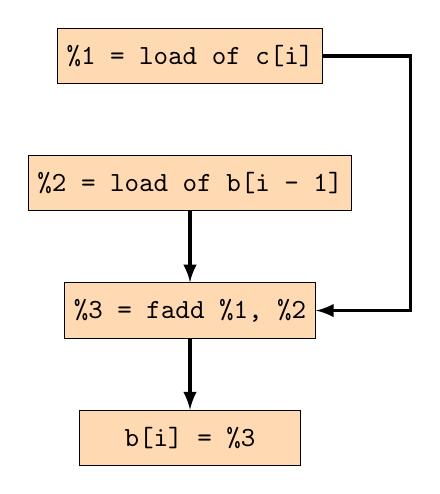
\begin{tikzpicture}[node distance = 9mm and 14mm,
  nodes= {draw, minimum width=8em, minimum height=2em, fill=orange!30,
    font=\ttfamily},
  arr/.style = {very thick,-latex}
  ]
  \node (var1) {\%1 = load of c[i]};
  \node (var2) [below=of var1] {\%2 = load of b[i - 1]};
  \node (var3) [below=of var2] {\%3 = fadd \%1, \%2};
  \node (var4) [below=of var3] {b[i] = \%3};

  \draw [arr] (var1) -- ++(2.8, 0) |- (var3);
  \draw [arr] (var2) -- (var3);
  \draw [arr] (var3) -- (var4);
\end{tikzpicture}
\end{document}
